\documentclass[11pt]{beamer}
\usepackage{amsmath, amsfonts, amscd, amssymb, amsthm, tikz,pgfplots}
\setbeamertemplate{navigation symbols}{}

\usepackage{caption}

\usetheme{eaperry}

\bibliographystyle{aer}
\usepackage{natbib}

\title{Initial Data Exploration}
\subtitle{LEED and Energy Star Data}
\institute{Spellman Program}
\author{Evan Perry}
\date{July 13, 2021}

\begin{document}

\maketitlepage

\begin{frame}{Review}

\begin{exampleblock}{\large\textbf{Research Question}}
What neighborhood characteristics relate to the number of certified energy-efficient commercial buildings?
\end{exampleblock}

\vfill
Previously,
\begin{itemize}
	\item Developed some theory behind energy-efficient building
	\item Prediction: Green buildings will be clustered away from the city center 
\end{itemize}

\end{frame}


\begin{frame}{Outline}

\begin{block}{Today's Goal}
Investigate available data on the number of certified energy-efficient (commercial) buildings from two major certification programs.
\end{block}

	\tableofcontents[hideallsubsections]
\end{frame}

\newsection{Background}{\textit{Introduction to the LEED and Energy Star Databases}}

\begin{frame}{Energy Star Program}

\begin{itemize}
	\item Program through the US Department of Energy and the Environmental Protection Agency
	\vfill

	\item Top 25\% for energy efficiency of comparable buildings
	\vfill
	
	\item Certified by a professional engineer or a special architect
	
	\vfill
	\item For federal agencies to lease space in a building, it must be Energy Star certified
\end{itemize}


\end{frame}


\begin{frame}{LEED Program}

\begin{itemize}
	\item Leadership in Energy and Environmental Design (LEED) program through the US Green Building Council
	\vfill
	
	\item Certification based  variety of ``green" criteria (e.g. energy-efficiency, facilities for electric cars \& bicycles)  
	\vfill

	\item Certified by a LEED accredited professional
\end{itemize}


\end{frame}

\newsection{Overview of Data Cleaning}{}

\begin{frame}{Data Cleaning}

\begin{minipage}{\textwidth}
\centering
\small
\captionof{figure}{Data Cleaning Process}

\begin{tikzpicture}[scale = .9]
	\draw[fill=EAPyellow,rounded corners] (0,2) rectangle (2,3.5) node[pos=.5]{$\substack{\text{Energy Star} \\ (37,783)}$};
	\draw[fill=EAPblue!60!,rounded corners] (0,0) rectangle (2,1.5) node[pos=.5]{$\substack{\text{LEED} \\ (160,159)}$};
	%\pause
	\draw[thick, ->] (2,0.75) -- (2.4, 0.75);
	\draw[thick, ->] (2,2.75) -- (2.4, 2.75);
	\draw[thick, ->] (2.2,0.75) -- (2.2, -1) -- (2.4, -1);
	\draw[fill=EAPyellow,rounded corners] (2.5,2) rectangle (4.5,3.5) node[pos=.5]{$\substack{\text{Clean}\\ \text{Energy Star} \\ (37,783)}$};
	\draw[fill=EAPblue!60!,rounded corners] (2.5,0) rectangle (4.5,1.5) node[pos=.5]{$\substack{\text{Clean LEED} \\ (100,807)}$};
	\draw[fill=lightgray, rounded corners] (2.5, -1.5) rectangle (4.5, -.5) node[pos=.5]{$\substack{\text{No U.S.} \\ \text{Address} \\ (59,352)}$};
	%\pause
	\draw[thick, ->] (4.5,0.75) -- (4.9, 1.25);
	\draw[thick, ->] (4.5,2.75) -- (4.9, 2.25);
	\draw[fill=EAPgreen, rounded corners] (5, .75) rectangle (7,2.75) node[pos=.5]{$\substack{\text{All Buildings} \\ (136,229)}$};
	\draw[fill=lightgray, rounded corners] (5,-1.5) rectangle (7,-.5) node[pos=.5]{$\substack{\text{Double}\\ \text{Counted} \\ (2,361)}$};
	\draw[thick,->] (6,.75) -- (6,-.4);
	%\pause
	\draw[thick, ->] (7,1.75) -- (9.9,1.75) node[pos =.5, above]{\scriptsize\textit{Geocoding}};
	\draw[thick, ->] (8.5, 1.75) -- (8.5, -1);
	\draw[fill=lightgray, rounded corners] (7.5,-.5) rectangle (9.5,-1.5) node[pos=.5]{$\substack{\text{Geocode}\\ \text{Failures} \\ (35,984)}$};
	\draw[fill = EAPgreen, rounded corners] (10,0.75) rectangle (12,2.75)  node[pos=.5]{$\substack{\text{Final Sample} \\ (100,245)}$};
\end{tikzpicture}
\bigskip

\footnotesize
(No. of Observations)
\end{minipage}

\end{frame}


\newsection{Visualizing the Data}{}

\begin{frame}{Energy Star Buildings}

\begin{figure}
	\caption{Sample of Energy Star Buildings by Type}
	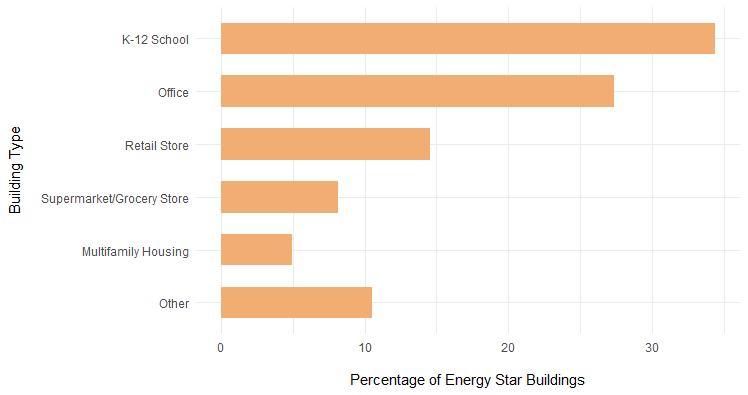
\includegraphics[width=\textwidth]{estar.png}
\end{figure}

\end{frame}


\begin{frame}{LEED Buildings}

\begin{figure}
\caption{Sample of LEED Buildings by Type}
	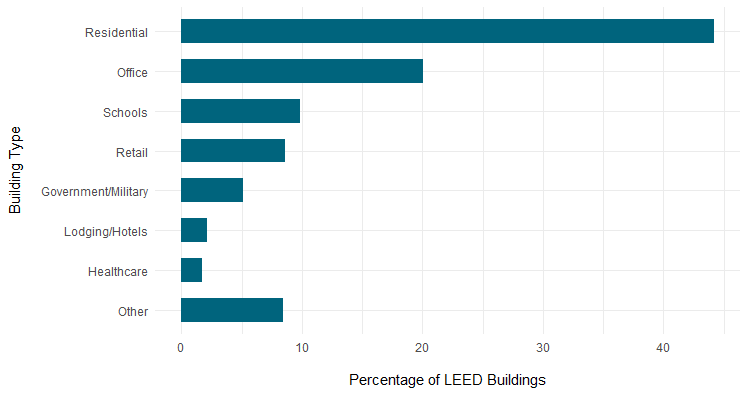
\includegraphics[width=\textwidth]{leed.png}
\end{figure}

\end{frame}


\begin{frame}{Where is the Sample?}

\begin{figure}
	\caption{Green Buildings by State}
	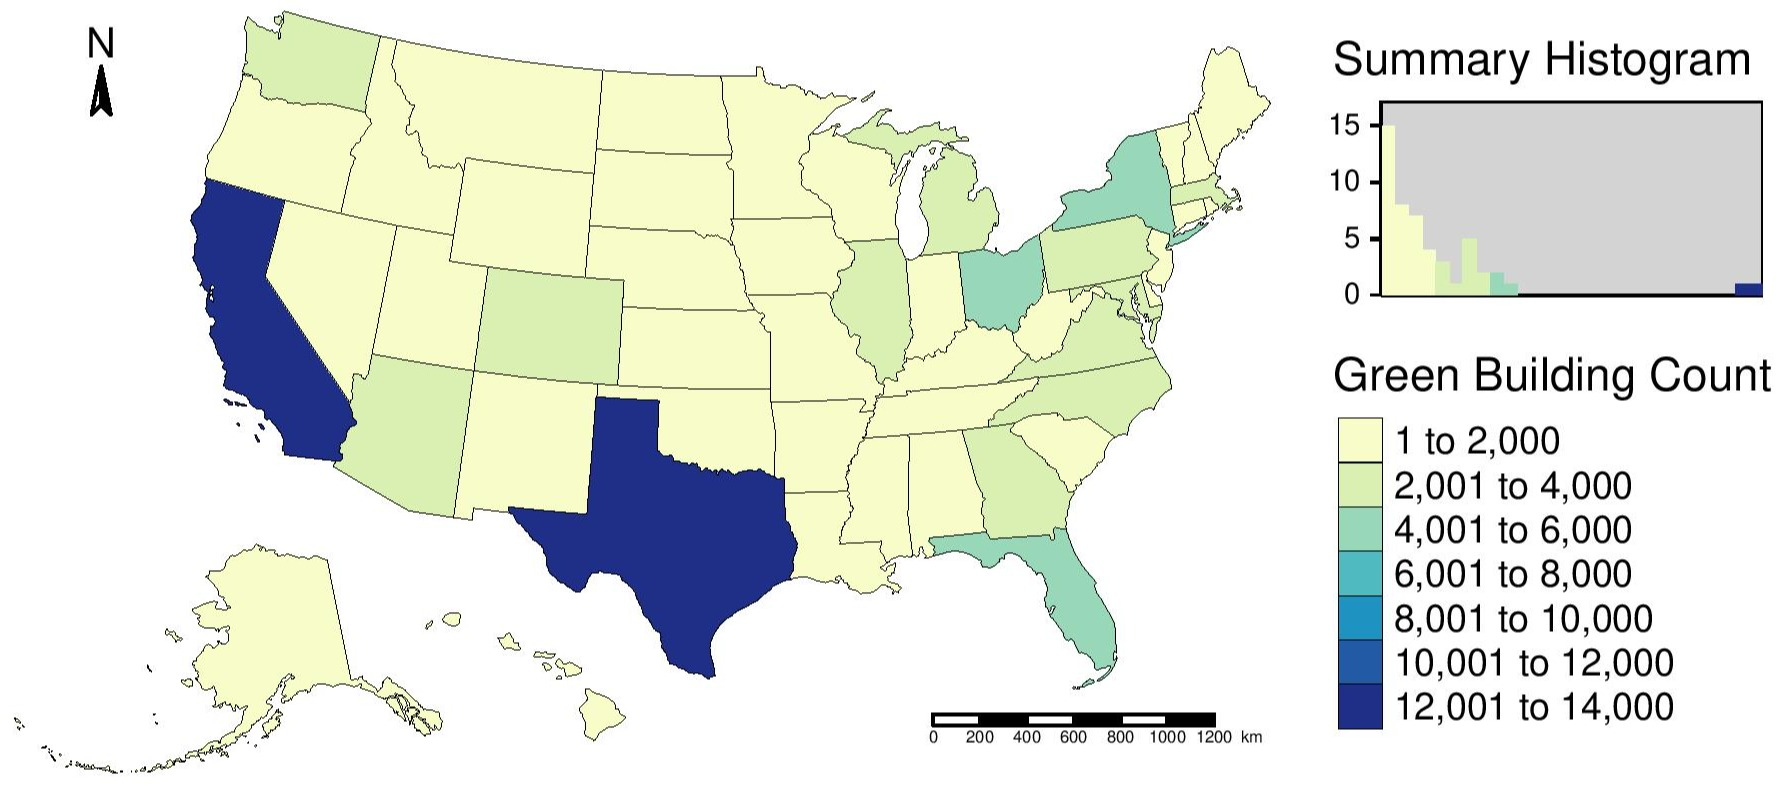
\includegraphics[width=\textwidth]{usCounts.jpg}
\end{figure}

\end{frame}

\begin{frame}{Normalizing by Population}

\begin{figure}
\caption{Green Buildings per Capita by State}
	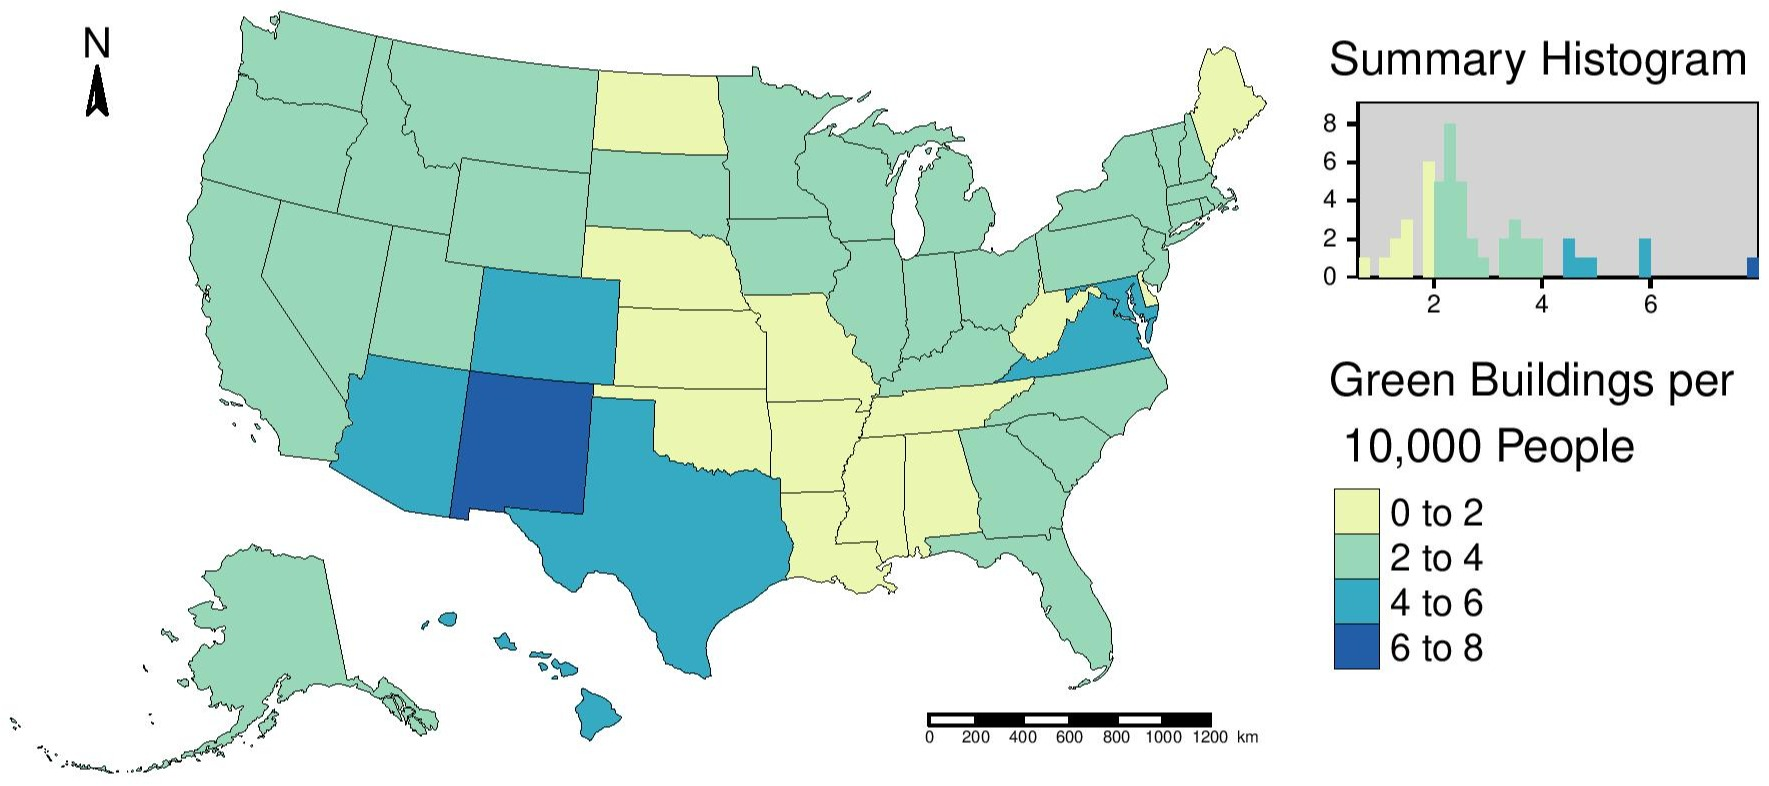
\includegraphics[width=\linewidth]{usCountsCapita.jpg}
\end{figure}

\end{frame}


\begin{frame}{Neighborhoods Around the Nation}

\begin{minipage}{\textwidth}
\captionof{table}{Summary Statistics}
\small
\centering
\begin{tabular}{l c c c}
\hline\hline\\ [-1.8ex]
Statistic & Full Sample & Commercial & Residential \\ 
\hline \\ [-1.8ex]
Total Count & 100,245 & 68,712 & 31,533\\ \\ [-1.8ex]
\textit{Census Tract Counts} \\ \\ [-1.8ex]
\quad Minimum & 0 & 0 & 0\\ \\ [-1.8ex]
\quad $25^\text{th}$ Pctl & 0 & 0 & 0\\ \\ [-1.8ex]
\quad Median & 0 & 0 & 0\\ \\ [-1.8ex]
\quad $75^\text{th}$ Pctl & 1 & 1 & 0\\ \\ [-1.8ex]
\quad Maximum & 458 & 154 & 456\\ \\ [-1.8ex]
\quad Mean & 1.376 & 0.943 & 0.433\\ \\ [-1.8ex]
\quad Count $\geq 1$ & 42.9\% & 39.0\% & 9.6\%\\
\hline
\end{tabular}
\end{minipage}


\end{frame}


\begin{frame}{Forming Counts}

\begin{figure}
	\caption{Green Buildings Counts, Hennepin County}
	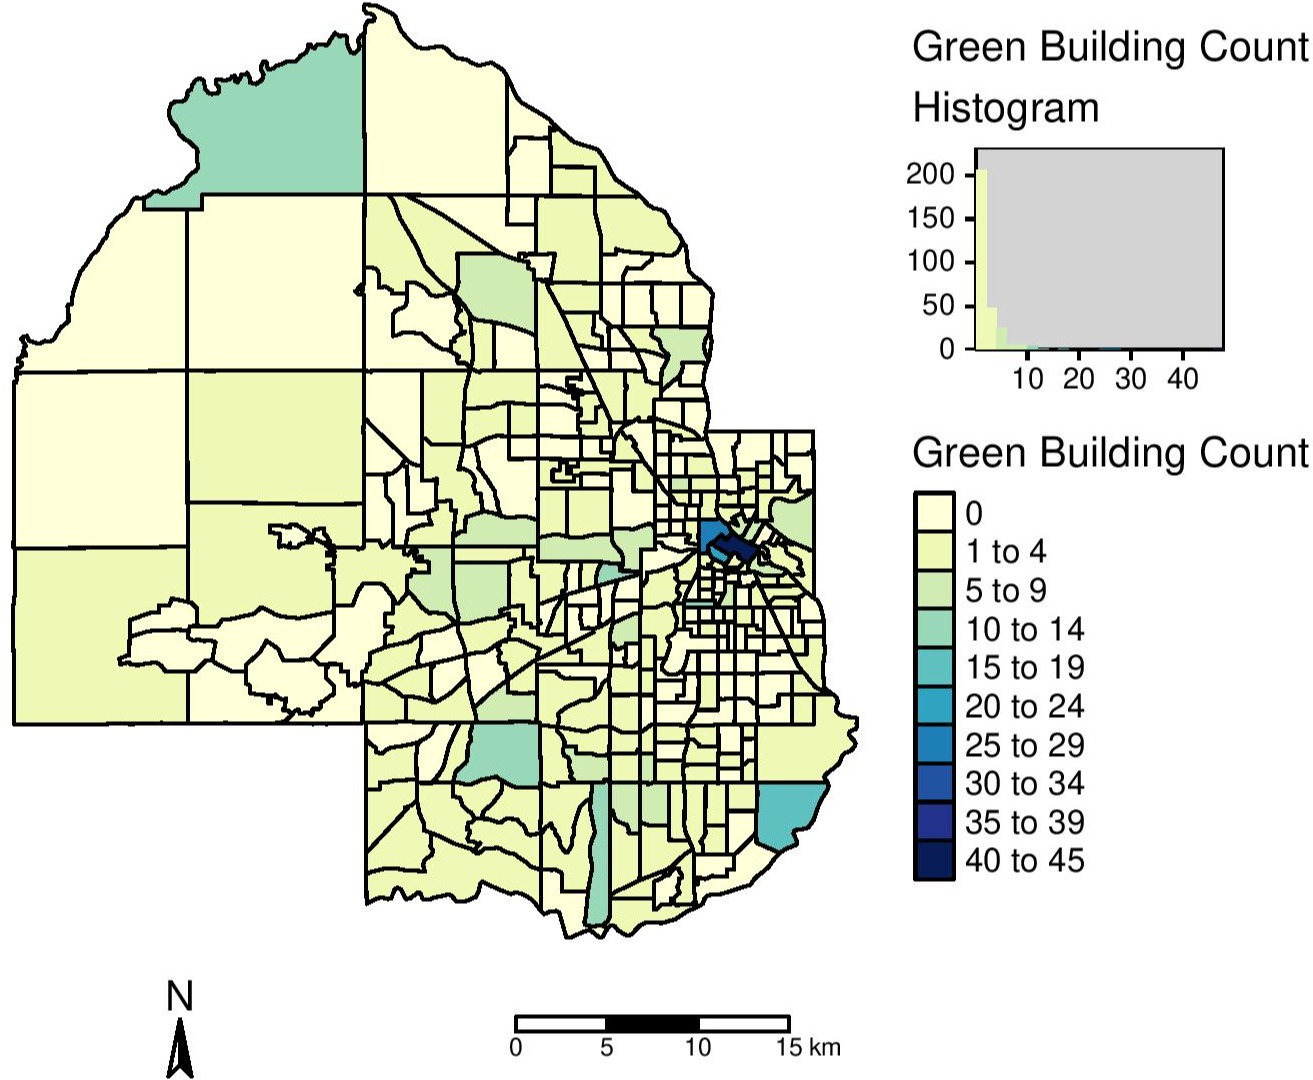
\includegraphics[width = 0.65\textwidth]{hCounts.jpg}
\end{figure}

\end{frame}


\begin{frame}{Next Week}

Revisit some theory: General equilibrium model for location of firms and workers.
\bigskip

{\bf Roback, Jennifer}, ``Wages, rents, and the quality of life,'' {\it Journal\\
 \quad of political Economy}, 1982, {\it 90} (6), 1257--1278.

\bigskip
{\bf Rosen, Sherwin}, ``Wage-based indexes of urban quality of life,'' \\
\quad {\it Current issues in urban economics}, 1979, pp.~74--104.

\end{frame}


%\begin{frame}{Plotting the Data}
%
%\begin{figure}
%	\caption{Green Buildings, Hennepin County}
%	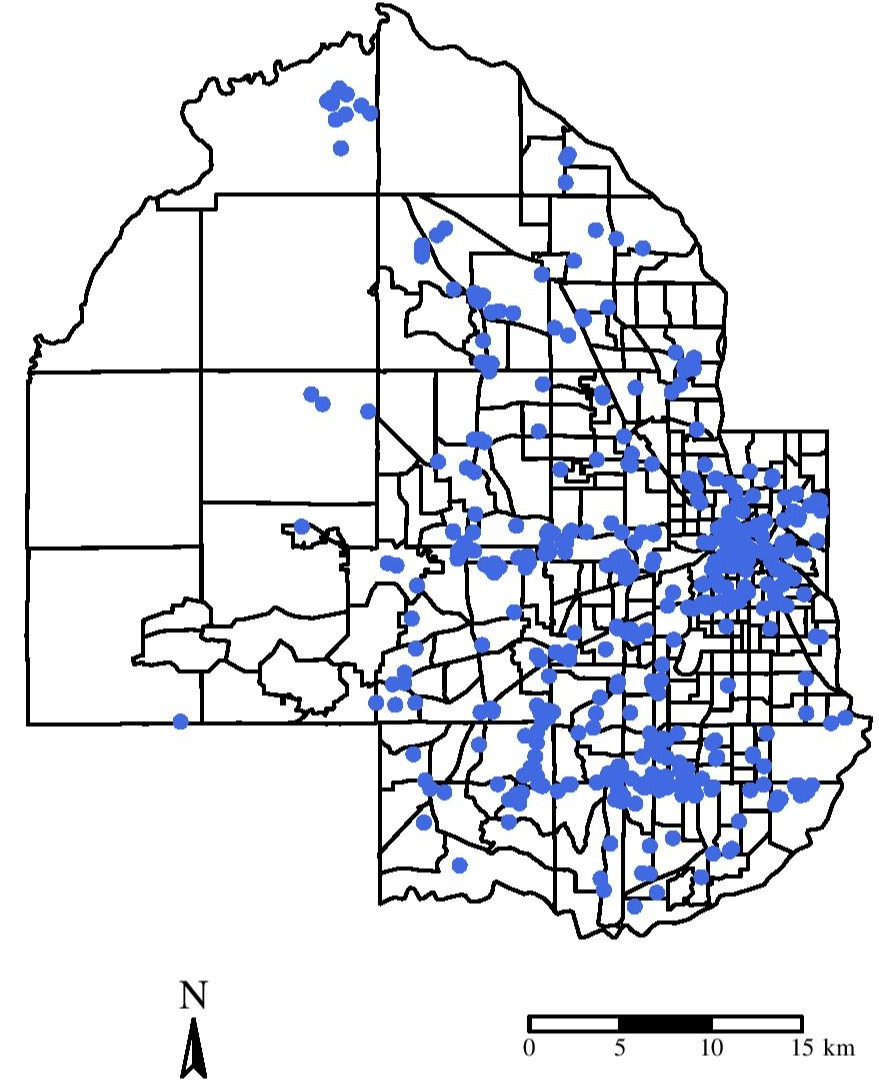
\includegraphics[width = 0.4\textwidth]{hPoints.jpg}
%\end{figure}
%
%\end{frame}


\end{document}